\documentclass[12pt,a4paper]{amsart}
\usepackage{amssymb}
\usepackage{listings}
\lstdefinelanguage{Macaulay2}
{morekeywords={for,from,if,do,while,apply,scan,print,method,help,viewHelp,table,exp,factor,needsPackage,ideal,det,determinan,res,coker,vars,Proj}, % TODO: use make-M2-symbols.m2
sensitive=false,
morecomment=[l]{--},
morecomment=[s]{-*}{*-},
morestring=[b]",
rulecolor=\color{blue!30},
}
\lstset{
  escapechar={`},
  aboveskip=0pt,
  belowskip=0pt,
  numbers=none,
  frame=leftline,
  framerule=1ex,
  framesep=1ex,
  xleftmargin=2ex,
  basicstyle={\ttfamily},
  columns=fixed,
  showstringspaces=false,
  commentstyle={\ttfamily\color{gray}},
  keywordstyle={\ttfamily\color{blue}},
  stringstyle={\ttfamily},
  fontadjust=true,
  basewidth={1.09ex},
  breaklines=false,
}
\usepackage[a4paper,left=2.25cm,right=2.25cm,top=3cm,bottom=3cm,headsep=1cm]{geometry}
\usepackage{tikz}%\usetikzlibrary{fit,positioning,matrix,calc,decorations.markings,angles,decorations.pathmorphing,decorations.pathreplacing}%,matrix,fit,shapes.geometric}
\title{Example file for M2inTeX}
\author{Paul Zinn-Justin}
\begin{document}
\maketitle

\section{Introduction}
some basic examples:
\smallskip
% start M2
\begin{lstlisting}[language=Macaulay2]
`\underline{i1}` : R=QQ[x,y]; factor(x^3-y^3)
\end{lstlisting}
\begin{lstlisting}[language=Macaulay2]
`\underline{o2}` = `$\left(x-y\right)\left(x^{2}+x\,y+y^{2}\right)$`
`\underline{o2}` : `$\texttt{Expression}$ of class $\texttt{Product}$`
\end{lstlisting}
% start M2
\begin{lstlisting}[language=Macaulay2]
`\underline{i3}` : res coker vars R
`\underline{o3}` = `$\underset{\vphantom{\Big|}0}{R^{1}}\,\xleftarrow{\left(\begin{smallmatrix}
x&y\\
\end{smallmatrix}\right)}\,\underset{\vphantom{\Big|}1}{R^{2}}\,\xleftarrow{\left(\begin{smallmatrix}
-y\\
x\\
\end{smallmatrix}\right)}\,\underset{\vphantom{\Big|}2}{R^{1}}\,\xleftarrow{0}\,\underset{\vphantom{\Big|}3}{0}$`
`\underline{o3}` : `$\texttt{ChainComplex}$`
\end{lstlisting}
% start M2
\begin{lstlisting}[language=Macaulay2]
`\underline{i4}` : OO_(Proj(R/(x^3-y^3)))^{1,2}
`\underline{o4}` = `${\mathcal O}_{\texttt{Proj}\left(\frac{R}{x^{3}-y^{3}}\right)}^{1}\left(1\right)\ \oplus \ {\mathcal O}_{\texttt{Proj}\left(\frac{R}{x^{3}-y^{3}}\right)}^{1}\left(2\right)$`
`\underline{o4}` : `coherent sheaf on $\texttt{Proj}\left(\frac{R}{x^{3}-y^{3}}\right)$, free`
\end{lstlisting}
\smallskip

more:
\smallskip
% start M2
\begin{lstlisting}[language=Macaulay2]
`\underline{i5}` : 318/46
`\underline{o5}` = `$\frac{159}{23}$`
`\underline{o5}` : `${\mathbb Q}$`
\end{lstlisting}
% start M2
\begin{lstlisting}[language=Macaulay2]
`\underline{i6}` : exp 3.73767
`\underline{o6}` = `${42}$`
`\underline{o6}` : `${\mathbb R}$ (of precision $53$)`
\end{lstlisting}
\smallskip

strings:
\smallskip
% start M2
\begin{lstlisting}[language=Macaulay2]
`\underline{i7}` : "hehe"
`\underline{o7}` = `hehe`
\end{lstlisting}
\smallskip

and nets: ({\tt tex Net} fixed on vanilla)
\smallskip
% start M2
\begin{lstlisting}[language=Macaulay2]
`\underline{i8}` : "haha"||"hoho"
`\underline{o8}` = `\begin{tabular}[t]{l}haha\\
hoho\end{tabular}`
\end{lstlisting}
\smallskip


\section{Help}
\smallskip
% start M2
\begin{lstlisting}[language=Macaulay2]
`\underline{i9}` : help det
`\underline{o9}` = `
\par \medskip\noindent\begingroup\Large\bf
determinant -- determinant of a matrix\endgroup
\par \smallskip%

\par \medskip\noindent\begingroup\Large\bf
Synopsis\endgroup
\par \smallskip%
\begin{itemize}
\item 
\par Usage: 
\par \begingroup\tt det\ M\endgroup{}
\item Inputs:\begin{itemize}
\item \begingroup\tt M\endgroup{}, a square \begingroup\tt matrix\endgroup{}
\end{itemize}

\item \begingroup\tt Optional\ inputs\endgroup{}:\begin{itemize}
\item \begingroup\tt Strategy\endgroup{}\begingroup\tt \ ={\char 62}\ \endgroup{}\begingroup\tt ...\endgroup{}, default value null, choose between Bareiss and Cofactor algorithms
\end{itemize}

\item Outputs:\begin{itemize}
\item a \begingroup\tt ring\ element\endgroup{}, which is the determinant of \begingroup\tt M\endgroup{}
\end{itemize}

\end{itemize}

\par \medskip\noindent\begingroup\Large\bf
Description\endgroup
\par \smallskip%

\par \medskip\noindent\begingroup\Large\bf
See also\endgroup
\par \smallskip%
\begin{itemize}
\item \begingroup\tt exteriorPower\endgroup{} -- exterior power
\item \begingroup\tt minors\endgroup{} -- ideal generated by minors
\item \begingroup\tt permanents\endgroup{} -- ideal generated by square permanents of a matrix
\item \begingroup\tt pfaffians\endgroup{} -- ideal generated by Pfaffians
\end{itemize}

\par \medskip\noindent\begingroup\Large\bf
Ways to use \begingroup\tt determinant\endgroup{} :\endgroup
\par \smallskip%
\begin{itemize}
\item \begingroup\tt {\char 34}determinant(Matrix){\char 34}\endgroup{}
\item \begingroup\tt {\char 34}determinant(MutableMatrix){\char 34}\endgroup{}
\end{itemize}

\par \medskip\noindent\begingroup\Large\bf
For the programmer\endgroup
\par \smallskip%

\par The object \begingroup\tt determinant\endgroup{} is a \begingroup\tt method\ function\ with\ options\endgroup{}.`
`\underline{o9}` : `$\texttt{DIV}$`
\end{lstlisting}
\smallskip


\section{packages}
packages that have a {\tt tex} output will work:
\smallskip
% start M2
\begin{lstlisting}[language=Macaulay2]
`\underline{i10}` : needsPackage "Posets";
\end{lstlisting}
% start M2
\begin{lstlisting}[language=Macaulay2]
`\underline{i11}` : booleanLattice 3
`\underline{o11}` = `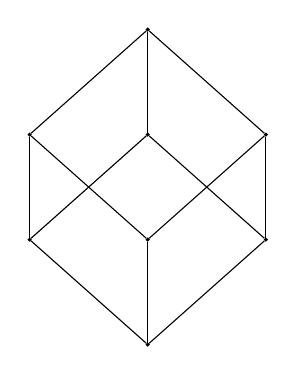
\begin{tikzpicture}[scale=1, vertices/.style={draw, fill=black, circle, inner sep=0pt}]
	\node [vertices] (0) at (-0+0,0){};
	\node [vertices] (1) at (-1.5+0,1.33333){};
	\node [vertices] (2) at (-1.5+1.5,1.33333){};
	\node [vertices] (4) at (-1.5+3,1.33333){};
	\node [vertices] (3) at (-1.5+0,2.66667){};
	\node [vertices] (5) at (-1.5+1.5,2.66667){};
	\node [vertices] (6) at (-1.5+3,2.66667){};
	\node [vertices] (7) at (-0+0,4){};
\foreach \to/\from in {0/1, 2/3, 0/2, 1/3, 4/5, 6/7, 4/6, 5/7, 0/4, 1/5, 2/6, 3/7}
\draw [-] (\to)--(\from);
\end{tikzpicture}
`
`\underline{o11}` : `$\texttt{Poset}$`
\end{lstlisting}
\smallskip


\section{multi-line example}
\smallskip
% start M2
\begin{lstlisting}[language=Macaulay2]
`\underline{i12}` : f = i -> (
      i+1
      )
`\underline{o12}` = `$\texttt{f}$`
`\underline{o12}` : `$\texttt{FunctionClosure}$`
\end{lstlisting}
\smallskip



\smallskip
% start M2
\begin{lstlisting}[language=Macaulay2]
`\underline{i13}` : I=ideal 0; f = i -> (
`\underline{o13}` : `$\texttt{Ideal}$ of ${\mathbb Z}$`
\end{lstlisting}
\begin{lstlisting}[language=Macaulay2]
   i+1)
`\underline{o14}` = `$\texttt{f}$`
`\underline{o14}` : `$\texttt{FunctionClosure}$`
\end{lstlisting}
\smallskip


\smallskip
% start M2
\begin{lstlisting}[language=Macaulay2]
`\underline{i15}` : a=1;b=2;
\end{lstlisting}
% start M2
\begin{lstlisting}[language=Macaulay2]
`\underline{i17}` : c=3;
\end{lstlisting}
\smallskip

That last one has no output

\end{document}
